\let\negmedspace\undefined
\let\negthickspace\undefined
\documentclass[journal]{IEEEtran}
\usepackage[a5paper, margin=10mm, onecolumn]{geometry}
%\usepackage{lmodern} % Ensure lmodern is loaded for pdflatex
\usepackage{tfrupee} % Include tfrupee package

\setlength{\headheight}{1cm} % Set the height of the header box
\setlength{\headsep}{0mm}     % Set the distance between the header box and the top of the text

\usepackage{gvv-book}
\usepackage{gvv}
\usepackage{cite}
\usepackage{amsmath,amssymb,amsfonts,amsthm}
\usepackage{algorithmic}
\usepackage{graphicx}
\usepackage{textcomp}
\usepackage{xcolor}
\usepackage{txfonts}
\usepackage{listings}
\usepackage{enumitem}
\usepackage{mathtools}
\usepackage{gensymb}
\usepackage{comment}
\usepackage[breaklinks=true]{hyperref}
\usepackage{tkz-euclide} 
\usepackage{listings}
% \usepackage{gvv}                                        
\def\inputGnumericTable{}                                 
\usepackage[latin1]{inputenc}                                
\usepackage{color}                                            
\usepackage{array}                                            
\usepackage{longtable}                                       
\usepackage{calc}                                             
\usepackage{multirow}                                         
\usepackage{hhline}                                           
\usepackage{ifthen}                                           
\usepackage{lscape}
\usepackage{circuitikz}


\author{EE25BTECH11041-Naman Kumar }
\graphicspath{./figs/}

\begin{document}
\begin{center}
    \huge{2.4.37}\\
    \large{EE25BTECH11041 - Naman Kumar}
\end{center}
Question:\\
Find a vector of magnitude 6, which is perpendicular to both the vectors $2\hat{\imath} - \hat{\jmath} + 2\hat{k}$ and $4\hat{\imath} - \hat{\jmath} + 3\hat{k}$\\
\solution \\
Cross of two vectors=\\
\begin{align}
\vec{A}\times\vec{B}=
\begin{pmatrix}
    |A_{23}&B_{23}|\\
    |A_{31}&B_{31}|\\
    |A_{12}&B_{12}|
\end{pmatrix}
\end{align}
And Magnitue or Length of any vecotr is,
\begin{equation}
\lVert \vec{A}\rVert=\sqrt{(\vec{A})^{T}(\vec{A})}
\end{equation}
Unit Vector in the direction of vector Perpendiculer to both A and B
\begin{align}
    \hat{C}=\frac{\vec{A}\times\vec{B}}{\lVert\vec{A}\times\vec{B}\rVert}
\end{align}
Given,
\begin{align}
    \vec{A}=\begin{myvec}{2\\-1\\2} \end{myvec},
    \vec{B}=\begin{myvec}{4\\-1\\3} \end{myvec}
\end{align}
By putting values in the equation
\begin{align}
    \vec{C}=\vec{A}\times\vec{B}=
    \begin{pmatrix}
        -1\times3-2\times-1\\
        2\times4 - 2\times3\\
        2\times-1-4\times-1
    \end{pmatrix}\\
    \vec{C}=\begin{pmatrix}
        -1\\
        2\\
        2
    \end{pmatrix}
\end{align}
Unit Vector is
\begin{align}
    \hat{C}=\frac{\vec{C}}{\lVert C \rVert}\\
    \hat{C}=\frac{1}{3}\begin{pmatrix} -1\\2\\2 \end{pmatrix}
\end{align}
Vector in the direction of $\pm\vec{C}$ with magnitude 6,
\begin{align}
    \vec{D}=\text{Magnitude}\times \text{Unit Vector}\\
    \vec{D}=\pm 6\times \frac{1}{3}\begin{pmatrix} -1\\2\\2 \end{pmatrix}
\end{align}
Therefore final vectors are
\begin{align}
    C_1=\begin{pmatrix} -2\\4\\4 \end{pmatrix},
    C_2=\begin{pmatrix} 2\\-4\\-4 \end{pmatrix}
\end{align}
\begin{figure}[H]
    \centering
    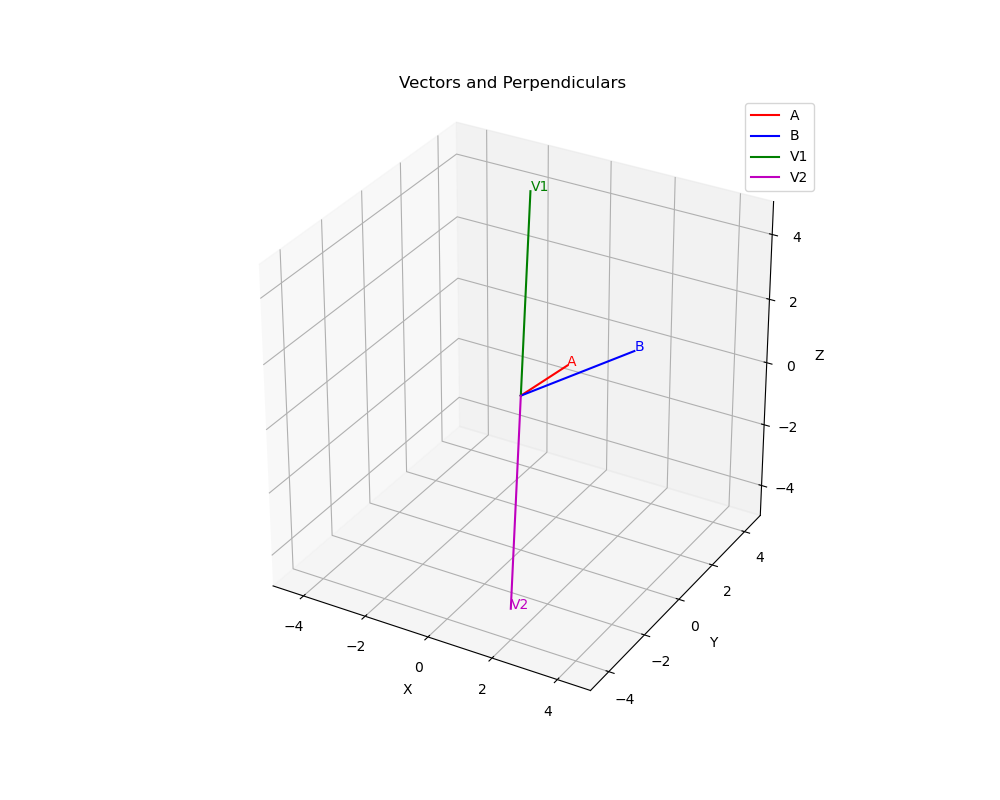
\includegraphics[width=\columnwidth]{figs/vector_plot.png}
    \caption{}
    \label{fig:placeholder}
\end{figure}

\end{document}
